%%%%%%%%%%%%%%%%%%%%%%%%%%%%%%%%%%%%%%%%%%%%%%%%%%%%%%%%%%%%%%%%%%%%%%%%%%%%
% AGUtmpl.tex: this template file is for articles formatted with LaTeX2e,
% Modified July 2014
%
% This template includes commands and instructions
% given in the order necessary to produce a final output that will
% satisfy AGU requirements.
%
% PLEASE DO NOT USE YOUR OWN MACROS
% DO NOT USE \newcommand, \renewcommand, or \def.
%
% FOR FIGURES, DO NOT USE \psfrag or \subfigure.
%
%%%%%%%%%%%%%%%%%%%%%%%%%%%%%%%%%%%%%%%%%%%%%%%%%%%%%%%%%%%%%%%%%%%%%%%%%%%%
%
% All questions should be e-mailed to latex@agu.org.
%
%%%%%%%%%%%%%%%%%%%%%%%%%%%%%%%%%%%%%%%%%%%%%%%%%%%%%%%%%%%%%%%%%%%%%%%%%%%%
%
% Step 1: Set the \documentclass
%
% There are two options for article format: two column (default)
% and draft.
%
% PLEASE USE THE DRAFT OPTION TO SUBMIT YOUR PAPERS.
% The draft option produces double spaced output.
%
% Choose the journal abbreviation for the journal you are
% submitting to:

% jgrga JOURNAL OF GEOPHYSICAL RESEARCH
% gbc   GLOBAL BIOCHEMICAL CYCLES
% grl   GEOPHYSICAL RESEARCH LETTERS
% pal   PALEOCEANOGRAPHY
% ras   RADIO SCIENCE
% rog   REVIEWS OF GEOPHYSICS
% tec   TECTONICS
% wrr   WATER RESOURCES RESEARCH
% gc    GEOCHEMISTRY, GEOPHYSICS, GEOSYSTEMS
% sw    SPACE WEATHER
% ms    JAMES
% ef    EARTH'S FUTURE
% ea    EARTH AND SPACE SCIENCE
%
%
%
% (If you are submitting to a journal other than jgrga,
% substitute the initials of the journal for "jgrga" below.)

\documentclass[draft,ms]{agutex}   %draft, [ms]
% To create numbered lines:

% If you don't already have lineno.sty, you can download it from
% http://www.ctan.org/tex-archive/macros/latex/contrib/ednotes/
% (or search the internet for lineno.sty ctan), available at TeX Archive Network (CTAN).
% Take care that you always use the latest version.

% To activate the commands, uncomment \usepackage{lineno}
% and \linenumbers*[1]command, below:

\usepackage{lineno}

\linenumbers*[1]
%  To add line numbers to lines with equations:
%  \begin{linenomath*}
%  \begin{equation}
%  \end{equation}
%  \end{linenomath*}
%%%%%%%%%%%%%%%%%%%%%%%%%%%%%%%%%%%%%%%%%%%%%%%%%%%%%%%%%%%%%%%%%%%%%%%%%
\usepackage{url}
\usepackage{amsmath}
\usepackage{rotating} 

\usepackage{lineno}
\usepackage[bottom]{footmisc}

\usepackage{graphics}

%\usepackage[dvips]{graphicx}
 
\usepackage{color}
\definecolor{pinkred}{rgb}{1.0, 0.4, 0.4}

% Author names in capital letters:
\authorrunninghead{HUANG ET AL.}

% Shorter version of title entered in capital letters:
\titlerunninghead{IRRIGATION IMPACTS IN VR-CESM}

%Corresponding author mailing address and e-mail address:
\authoraddr{Corresponding author: Xingying Huang,
Department of Land, Air and Water Resources, \\
 University of California Davis, Davis, CA 95616, USA.
 (xyhuang@ucdavis.edu)}
 
%Department of Hydrology and Water Resources, University of
%Arizona, Harshbarger Building 11, Tucson, AZ 85721, USA.
%(a.b.smith@hwr.arizona.edu)}

\begin{document}

%% ------------------------------------------------------------------------ %%
%
%  TITLE
%
%% ------------------------------------------------------------------------ %%


\title{Irrigation impacts on California's climate with the variable-resolution CESM}

%A study of 

%
% e.g., \title{Terrestrial ring current:
% Origin, formation, and decay $\alpha\beta\Gamma\Delta$}
%

%% ------------------------------------------------------------------------ %%
%
%  AUTHORS AND AFFILIATIONS
%
%% ------------------------------------------------------------------------ %%

%Use \author{\altaffilmark{}} and \altaffiltext{}

% \altaffilmark will produce footnote;
% matching \altaffiltext will appear at bottom of page.

% \authors{A. B. Smith,\altaffilmark{1}
% Eric Brown,\altaffilmark{1,2} Rick Williams,\altaffilmark{3}
% John B. McDougall\altaffilmark{4}, and S. Visconti\altaffilmark{5}}

%\altaffiltext{1}{Department of Hydrology and Water Resources,
%University of Arizona, Tucson, Arizona, USA.}

%\altaffiltext{2}{Department of Geography, Ohio State University,
%Columbus, Ohio, USA.}

%\altaffiltext{3}{Department of Space Sciences, University of
%Michigan, Ann Arbor, Michigan, USA.}

%\altaffiltext{4}{Division of Hydrologic Sciences, Desert Research
%Institute, Reno, Nevada, USA.}

    \authors{Xingying Huang,\altaffilmark{1}
  Paul A. Ullrich, \altaffilmark{1} }

\altaffiltext{1}{Department of Land, Air and Water Resources, University of California, Davis}


%%%%%%%%%%%%%%%%%%%%%%%%%%%%%%%%%%%%%%%%%%%%%%%%%%%%%%%%%%%%%%%%%%%%%
% ABSTRACT
%
% Enter your Abstract here

\begin{abstract}

The variable-resolution capability within the Community Earth System Model (VR-CESM) is applied to understand the impact of irrigation on the regional climate of California. Irrigation is an important contributor to the regional climate of heavily irrigated regions, and within the U.S. there are few regions that are as heavily irrigated as California's Central Valley, responsible for 25$\%$ of domestic agricultural products. A flexible irrigation scheme with relatively realistic estimates of agricultural water use is employed. The impact of irrigation on mean climatology and heat extremes is investigated over the 26 year period 1980-2005 using a relatively fine grid resolution of $0.25^\circ$ ($\sim$28 km). Three simulations are performed, including an unirrigated control run and two irrigation-enabled runs, with results compared to gridded observations and weather station datasets. During the summer months (when irrigation peaks), irrigation leads to cooling of the daily maximum near-surface temperature field (Tmax) by approximately 1.1 K. Under irrigation, latent heat flux increased by $\sim$61$\%$ during the daytime as a result of increased surface evaporation; specific humidity increased by about 12$\%$; heat stress was reduced by 22$\%$ and the average soil moisture exhibited a small ($\sim$4.4$\%$) but statistically significant increase. Compared with observations, irrigation improved the frequency distribution of Tmax, and both length and frequency of hot spells were better represented with irrigation enabled. Consequently, we argue that high-resolution simulations of regional climate in CESM, particularly over heavily irrigated regions, should likely enable the irrigation parameterization to better represent local temperature statistics.


\end{abstract}


\begin{article}


%%%%%%%%%%%%%%%%%%%%%%%%%%%%%%%%%%%%%%%%%%%%%%%%%%%%%%%%%%%%%%%%%%%%%
% MAIN BODY OF PAPER
%%%%%%%%%%%%%%%%%%%%%%%%%%%%%%%%%%%%%%%%%%%%%%%%%%%%%%%%%%%%%%%%%%%%%
%
\section{Introduction}

Over the past century, human activity has had a clear impact on global and regional climate, largely through indirect effects associated with increasing greenhouse gases \citep{solomon2007ipcc}, but also as a result of land cover changes, particularly deforestation, agriculture and urbanization \citep{bonan1997effects, pielke2002influence, kueppers2008seasonal}. Conversion of the natural land cover to cropland features prominently in this change, which is accompanied by modified albedo and differences in both sensible and latent heat fluxes \citep{foley2003green}. Besides affecting energy balance, land management also impacts the climate system by modifying the carbon and water cycles, which are driven in part by cropping length and irrigation strategy \citep{lobell2006biogeophysical}. The pronounced cooling effect of irrigation, especially over regions where irrigation is extensive, has been emphasized by previous studies \citep{kueppers2007irrigation, lobell2008effect}.

California is the most irrigated state in the U.S., and most of California's irrigated cropland is distributed over the Central Valley (CV), which is responsible for 25$\%$ of domestic agricultural products \citep{wilkinson2002preparing}. The CV extends 600 km between its northernmost and southernmost point and is between 60-100km in width.  It features a vast agricultural industry that has adapted to an extremely dry growing season with a Mediterranean climate through the adoption of extensive irrigation practices. The USGS reported that in the year 2000, approximately 42 km$^3$ of water was used over $\sim$41,000 km$^2$ of irrigated area within California \citep{doll2002global, famiglietti2011satellites}. \cite{bonfils2007empirical} found that irrigation over CV has decreased summertime maximum temperature by $\sim$2-3 K in heavily-irrigated areas compared with nearby non-irrigated areas, based on long-term temperature records, although these impacts had a negligible effect on nighttime temperatures. Similar impacts have also been demonstrated in Nebraska's irrigated areas by \citet{mahmood2006impacts}.

However, irrigation effects are usually ignored in climate models for several reasons: irrigation usually occurs over a relatively small area ($\sim$2$\%$ of global land surface) and produces a seemingly negligible cooling effect compared to global greenhouse warming \citep{boucher2004direct}. Nonetheless, irrigation is a potentially important factor in regulating climate patterns at regions scales, where there is a growing need for accurate climate assessments and projections. Past studies have typically addressed the climatic effects of irrigation in limited-area models (LAMs) \citep{snyder2006regional, kueppers2007irrigation}, which in the context of climate modeling are typically referred to as regional climate models (RCMs). In these studies, irrigation is modeled by accounting for the amount of irrigated water needed and the area of cropland where irrigation is applied. Using a multi-model ensemble of RCM simulations, \cite{kueppers2008seasonal} found that the behavior of RCMs varied in representing effects of irrigation on regional climate, depending on each model's physics, as well as on the configuration of the irrigation parameterization.

Although global climate models (GCMs) rarely account for irrigation, it is nonetheless meaningful to understand to what extent irrigation may affect the global climate patterns \citep{sacks2009effects}. \citet{lobell2006biogeophysical} coupled the community atmosphere model (CAM) 3.0 to the community land model (CLM) 3.0 at $\sim$2-2.5$^\circ$ horizontal grid spacing to model irrigation by fixing soil moisture at saturation during the growing season in all croplands. Although this approach likely overcompensated for total added water, it produced global land surface cooling of 1.3 K, and regional cooling of up to 8 K. \citet{lo2013irrigation} used CAM 3.5 along with CLM 3.5 at $\sim$1.4$^\circ$ horizontal resolution, and argued that the increase in evapotranspiration and water vapor due to irrigation significantly impacts the atmospheric circulation in the southwestern United States by strengthening the regional hydrological cycle.

The aforementioned studies either used RCMs or coarse-resolution GCMs, along with different irrigation parameterizations. In order to model regional climate over the CV, relatively fine horizontal resolution is needed to more accurately represent microclimates, land-use, small-scale dynamical features and corresponding interactions \citep{leung2003regional, rauscher2010resolution}. In this paper, we use the recently developed variable-resolution option in Community Earth System Model (VR-CESM) to study the impact of irrigation on regional climate over the CV, that features a more flexible irrigation scheme with relatively realistic estimates of regional agricultural water use (as will be described in Section 2). Variable-resolution GCMs (VRGCMs) such as VR-CESM use a relatively coarse global model with enhanced resolution over a specific region \citep{staniforth1978variable, fox1997finite}. 


Compared with RCMs, a key advantage of VRGCMs is that they use a single, unified modeling framework, rather than a separate GCM and RCM with potentially inconsistent dynamics and physics parameterizations and lack of two-way interactions at the nest boundary \citep{laprise2008challenging}. When compared to uniform-resolution global models, VRGCMs provide a cost-effective approach for reaching high resolutions over a region of interest -- the regional simulations in this study at 0.25$^\circ$ ($\sim$28 km) resolution represent a reduction in required computation of approximately 10 times over a global uniform simulation with resolution of 0.25$^\circ$. VR-CESM has been demonstrated to be effective for regional climate studies and applications at a reduced computational cost compared to uniform GCMs \citep{zarzycki2015effects, rhoades2015characterizing, huang2016evaluation}. In particular, this study is one of the first to use variable resolution for assessing the impact of a physical parameterization at high-resolution in a global Earth-system model. The central hypothesis of this paper is that irrigation in the CV of California is an important contributor to the region's surface energy budget and must be accounted for in order to properly simulate temperature statistics, tested by a control (non-irrigated) and two irrigated 26-year simulations in VR-CESM.

This work builds on a number of previous modeling studies that have explored the importance of irrigation in controlling the climate over the CV region in the following ways: (1) it employs relatively high resolution ($\sim$28 km) covering the western U.S. over long-term period  (from year 1980-01-01 to 2005-12-31); (2) it uses a more realistic irrigation parameterization embedded in CLM 4.0 and coupled in CESM 1.2.0 rather than experimentally fixed irrigated water, as in many previous studies (\textit{i.e.} \cite{lobell2006biogeophysical, lo2013irrigation}); (3) it uses a variable-resolution global climate model (rather than the low-resolution global or limited area models forced by reanalysis dataset or GCM output that have been previously used); and (4) it explores a more comprehensive array of impacts of irrigation on the regional climate, focusing on temperature statistics, including extreme heat episodes.  We conclude that the irrigation parameterization in CESM is effective at addressing a bias in daily maximum temperatures and heatwave statistics in California's CV, and is necessary in order to accurately capture temperature statistics in heavily irrigated regions at high model resolution.

This paper is organized as follows: Section 2 describes the model setup, employed datasets and methodology. In section 3, simulation results are provided and analyzed. Key results are summarized along with further discussion in section 4.

\section{Model setup and reference datasets}

\subsection{Irrigation parameterization}

As a state-of-the-art Earth modeling framework, CESM 1.2.0 consists of coupled atmospheric, oceanic, land and sea ice models \citep{CAM5Tech, hurrell2013community}. In this study, CAM version 5 (CAM5) \citep{CAM5Tech} and CLM version 4.0 \citep{CLM40Tech} are used.  Global sea-surface temperatures are prescribed in accordance with the Atmospheric Model Intercomparison Project (AMIP) protocol \citep{Gates1992}.  The finest horizontal resolution of our grid is $\sim$28 km covering the western U.S., with a quasi-uniform 1$^\circ$ mesh over the remainder of the globe (see Figure \ref{fig:Figure 1}). Considering the relatively flat topography (less than 100 m) over most of CV, the $\sim$28 km grid resolution satisfies our need for modeling irrigation effects. In particular, simulations at 0.125$^\circ$ ($\sim$14 km) conducted in \cite{huang2016evaluation} did not show a statistically significant change in temperature statistics over California.  In our study, as in \cite{zarzycki2015effects}, general circulation patterns (e.g., wind, pressure and precipitation) do not exhibit apparent artifacts in the variable-resolution transition region. A detailed description of the techniques of VR-CESM employed in this paper can be found in \cite{rhoades2015characterizing}. Here, our model description focuses on the irrigation scheme within CLM 4.0.

The fractional land-use data used for computing cropland (independent of specific type) that is equipped for irrigation within each grid cell is from \citet{siebert2005development} for the year 2000, and is fixed over the simulation period (see Figure \ref{fig:Figure 2}). This assumption is reasonable since irrigated area has been largely unchanged in California since year 1980 \citep{bonfils2007empirical}. 

The need for daily irrigation is determined at 6 AM local time by computing the deficit between the current soil moisture content and a target soil moisture content.  Note that this calculation does not account for the infiltration rate of the soil. If positive, the difference is then added to the ground surface at a constant rate over the following four hours, bypassing canopy interception. By default, CLM simulates ten soil layers, with a total depth of 3.4 m \citep{CLM40Tech}. The target soil moisture content in each soil layer $i$ ($w_{target, i}$, in kg/m$^2$) is a weighted average of (a) the minimum soil moisture content that results in no water stress (w$_{o,i}$, kg/m$^2$) and (b) the soil moisture content at saturation ($w_{sat,i}$, kg/m$^2$), in accordance with

\begin{align} \label{eq:TargetSoilMoisture}
w_{target,i} = (1-{\alpha})*w_{o,i} + {\alpha}*w_{sat,i}
\end{align} The default value of the irrigation weight factor $\alpha$ is 0.7, which was determined empirically to give global, annual irrigation amounts that approximately match observed gross irrigation water use around the year 2000 \citep{shiklomanov2000appraisal}. This parameterization is designed to approximate human behavior -- that is, enough water is added so as to avoid water stress in crops, but not so much that the soil is completely saturated. More details about the irrigation model can be found in the online technical description \citep{irrigationTechnicCLM}.

\subsection{Simulations}

In order to understand the impacts on the local climate triggered by irrigation over the CV, we have conducted a control run (NRG) without irrigation and two irrigation-enabled runs, referred to as IRG and IRG(0.5) respectively. The IRG run uses the default irrigation weight factor ($\alpha = 0.7$).  This value was adjusted to 0.5 in the irrigated IRG(0.5) run so as to determine the impact of changes in total irrigation water. Simulations were performed over the period 1979-01-02 to 2005-12-31 (UTC).  For purposes of analysis, 1979 was discarded as a spin-up period to allow adequate time for the land and atmosphere to equilibrate.  Initial soil moisture conditions are specified from the output of long-term simulations so as to ensure the groundwater aquifer was initially in near-equilibrium with the local climatology. The 26-year time period was chosen to provide an adequate sampling of annual variability within computational constraints. A land cover dataset at 3 min ($\sim$10 km) grid resolution for year 2000 was used as it provided a realistic fraction of irrigated cropland in each grid cell over the CV when interpolated onto the 28 km grid (see Figure 2). 

Irrigation water applied in the IRG simulation was $\sim$2.84 mm/day in JJA when averaged over the CV, which equates to 31.7 km$^3$ total water. Given that no reliable and comprehensive dataset on cropland utilization or fallowing is available, and that information on local irrigation practices is even harder to come by, it was determined that there was no precise and publicly available numbers for the irrigation area and total utilized irrigation water over the CV. However, as mentioned earlier, in the year 2000 the USGS reported that approximately 42 km$^3$ of water was used over approximately 41,000 km$^2$ of irrigated area in California. Based on the fraction of cropland equipped for irrigation in the year 2000 obtained from \citet{siebert2005development}, we arrived at an estimate of CV irrigated area of about 33,190 km$^2$, which is about 81$\%$ of California's total irrigated area.  Assuming between half to two thirds of the 42 km$^3$ of water was employed over the CV during JJA (excluding certain water amount for late spring and early fall), that resolves to about 21 to 28 km$^3$, or 0.66 to 0.88 times the amount applied in IRG ($\sim32 \mbox{km}^3$). This suggests that the water use imposed by this irrigation scheme is relatively realistic.


\section{Methodology}

In the CV, irrigation peaks during the summer growing season \citep{salas2006estimating} in response to California's dry Mediterranean summers (with a precipitation rate of about 0.13 mm/day averaged over year 1980-2005). Our simulations accurately reproduce this observation, as most irrigated water is added during summer (see Figure 1 in the supplement document). To study the  climatological impacts of irrigation, we focus primarily on changes in June, July and August (JJA) near-surface (2 m) temperatures including daily maximum, minimum and average temperatures (Tmax, Tmin and Tavg), and the associated mechanisms driving the relative changes. 

To determine how irrigation affects heat extremes within the CV, we calculated hot spell length, hot spell frequency, and mean Tmax over the hot spells, based on the JJA daily Tmax over the 1980-2005 period. For our purposes, a hot spell is present in a given grid cell when five or more consecutive days with Tmax exceeds 38$^\circ$C. This threshold value approximately corresponds to the 90th percentile of all daily Tmax values within the CV. \textit{Hot spell length} is defined as the average duration (in days) for all  hot spells over the 26 year period, \textit{hot spell frequency} is defined as the average number of hot spells per year, and \textit{mean hot spell Tmax} is defined as the average Tmax over all the hot spell days. When analyzing hot spells, declustering is employed following the strategy of \cite{ferro2003inference} to ensure hot spells are serially independent.  This functionality is implemented in the R package \texttt{extRemes} \citep{gilleland2011new}.

To restrict the analysis to the CV, the variables of interest have been masked and/or averaged within the area defined by the bounded region as sketchily depicted in Figure \ref{fig:Figure 2}, which contains 155 grid points. To quantify model performance against reference datasets, the root-mean-square deviation (RMSD) and mean signed difference (MSD) are used, and spatial correlation (Corr) is assessed by computing sample linear cross-correlations at lag 0 after converting a two-dimensional dataset to a one-dimensional array. Mathematically, RMSD and MSD are written as, 

\begin{align}
RMSD &= \sqrt{\frac{1}{N} \sum_{i=1}^{N} (v_i - \hat{v}_i)^2}  & MSD &= \frac{1}{N} \sum_{i=1}^{N} (v_i - \hat{v}_i) 
\end{align} where $v_i$ and $\hat{v}_i$ are values from the simulation output and reference dataset respectively; $i$ is the grid-point index and N is the total number of grid points over specific regions.

Throughout the remainder of this paper, Student's t-test has been used to test the equality of the means of two datasets. This is employed for the seasonally-averaged data at each grid point and for spatially averaged data over CV. F-test is applied to test whether the sample variances are equal. These tests are used here when the sample population can be adequately described by a normal distribution, where normality is assessed under the Anderson-Darling test. All these tests are evaluated at the $\alpha = 0.05$ significance level. 

\subsection{Reference datasets}

For comparison, we employ two high-quality gridded observational datasets (UW and PRISM) and selected weather station data (NCDC) to evaluate our simulation output. The detailed descriptions of these reference datasets are as follows.

\paragraph{UW} The UW daily gridded meteorological data is obtained from the Surface Water Modeling group at the University of Washington \citep{maurer2002long, hamlet2005production}. The dataset is provided at 0.125$^\circ$ horizontal resolution covering the period from year 1949 to 2010 with daily time frequency for Tmax and Tmin in the aspect of temperature, which are used in this study.

\paragraph{PRISM} The Parameter-elevation Regressions on Independent Slopes Model (PRISM) \citep{daly2008physiographically} gridded dataset at 4 km resolution is also employed in this study.  This model ingests point measurements and applies a weighted regression scheme that accounts for key factors affecting the local climatology. PRISM is the United States Department of Agriculture's official climatological dataset. Monthly climatological variables are available for year 1895 through 2015 and daily data for year 1981 to 2015 from the PRISM Climate Group \citep{prismSource}. This study makes use of monthly Tmax, Tmin, Tavg, and daily Tmax.

\paragraph{NCDC} Weather station measurements over the CV are obtained from the Global Historical Climate Network (GHCN) and provided by NOAA/NCDC \citep{menne2012overview}. Weather stations within the study region were chosen from all stations with at least 90$\%$ observations of Tmax over all JJA days from 1981 to 2005.  A subset of 11 stations were then chosen to provide roughly even spatial coverage of the CV.

\section{Results}

The average JJA Tmin, Tavg and Tmax over the 1980-2005 period from all simulations and gridded datasets are depicted in Figure \ref{fig:Figure 3}. Relative to the gridded datasets, NRG has a prominent overestimation of Tmax, with MSD values of $\sim$0.75 K and RMSD values of $\sim$1.7 K (see Table \ref{tab:table1}). The cooling effect caused by irrigation is clear in all temperature fields when comparing NRG and IRG results, with all fields exhibiting significant differences over parts of the CV (as hatched in Figure 3). Notably, no statistically significant difference in temperature arises from reducing the irrigation factor from 0.7 to 0.5. Although the IRG run shows a slight cold bias with an MSD around -0.36 K (which is reduced in IRG(0.5) to around -0.2 K), this effect is limited to the base of the Sierra Nevada and the San Francisco Bay Delta region.

Compared with NRG, the RMSD of Tmax for IRG(0.5) is only reduced by about 20$\%$ against PRISM, which appears to be due to the offset effects caused by the non-irrigated grid cells around our study region's boundary. Although Tmin was also reduced by about 0.5 K in IRG over the irrigated area, all three runs still exhibit a warm bias in this field relative to the reference. The net result is that Tavg is overestimated in NRG over the CV, except in regions influenced by the Delta sea breeze, whereas IRG produced a slight cool bias in Tavg after alleviating the overestimation of Tmax in the northern and southern reaches of the CV. The correlation coefficients between simulations and reference datasets are about 0.76 to 0.86, indicating that VR-CESM can capture the overall spatial distributions of temperature. Although NRG and IRG are highly correlated with each other ($>$0.95), this simply implies that the spatial pattern of IRG is quite similar to NRG under spatially uniform cooling. Over non-irrigated areas, the results are essentially identical among all runs, suggesting that temperature modulation is largely a local phenomenon.

As mentioned earlier, the differences {\color{red}in temperature} between the IRG and IRG(0.5) simulations were not statistically significant, and were much smaller than the differences between IRG and NRG. Therefore, the intrinsic variability (even with some differences in irrigation water amounts) is small for VR-CESM relative to the effect of irrigation. This further testifies that the statistically significant differences between IRG and NRG are due to enabled irrigation instead of random variation.

%The overall performance of VR-CESM in modeling regional climate is out of the scope of this study, but has been extensively discussed in \citep{huang2016evaluation}.

Key variables associated with the irrigation model have been tabulated in Table \ref{tab:table2}. Tmax, latent heat flux, precipitation and soil moisture are further illustrated in Figure \ref{fig:Figure 4}. With the relative scarcity of natural precipitation in summer season ($\sim$0.1 mm/day), there is a $\sim$61\% increase in latent heat flux after adding $\sim$2.84 mm/day irrigated water for IRG over the hot and dry summer period. The main contribution to latent heat flux increase from NRG to IRG is due to ground evaporation (which is about 2.5 times larger), as vegetation evapotranspiration did not differ significantly between NRG ($\sim$1.1 mm/day) and IRG ($\sim$1.25 mm/day). Therefore, cooling of Tmax is largely due to increased latent heat flux during the daytime caused by evaporation from the surface. 

With irrigation enabled, the specific humidity increased by about 12$\%$ due to increased evaporation, and sensible heat flux decreased by 13\% with lower surface temperatures and a shift of sensible to latent heat flux. The soil moisture averaged over all surface and subsurface soil layers showed a statistically significant increase ($\sim4.4\%$) under irrigation. Since variability of the soil moisture is smaller at lower levels compared to upper levels, even a 4.4$\%$ change in the total column average was significant.  The change in soil moisture was largest near the surface, with soil water in the topmost five soil layers increased by more than 10$\%$ (reaching $\sim52\%$ at the first thin layer).


Notably, the small difference in column soil moisture (averaged over all the ten soil layers) between IRG and IRG(0.5) (equal to about 1.4$\%$, but still significant at the 95\% level) suggests that irrigated water does not effectively infiltrate into lower soil layers, given that the irrigated water applied in IRG is more than two times that of IRG(0.5). The soil water between IRG and IRG(0.5) is significantly different at the ground surface ($\sim5\%$ difference) and in the bottom layers ($\sim1\%$ difference), but not at the near-surface and throughout the middle levels. In fact, most of the additional water ($\sim$1.57 mm/day) from IRG(0.5) to IRG directly led to surface runoff (parameterized by removing surface water after infiltration into the soil at $\sim$0.24 mm/day for IRG(0.5) and $\sim$1.6 mm/day for IRG). Since irrigation water use in the IRG simulations is comparable to observations, this suggests that ineffective infiltration could be driving substantial water waste in the CV.


Based on the JJA-averaged values of each year over the 26-year period, box-and-whisker diagrams for four selected variables are given in Figure \ref{fig:Figure 4}. With irrigation, both the average magnitude and annual variability of Tmax (around 0.9$^\circ$C) are closer to observations. Compared to NRG, the range of Tmax for irrigation runs reduced to $\sim$3$^\circ$C from $\sim$4.5$^\circ$C with a more concentrated distribution, suggesting that there may be some indication of irrigation having a modulating effect on temperature variability (although the differences of variances are not statistically significant). The mean latent heat flux almost doubles when irrigation in enabled, however the variance of the distribution (with inter-annual {\color{red}standard deviation} of $\sim$2.7 $W/m^2$ for IRG and $\sim$3.3 $W/m^2$ for IRG(0.5)) did not substantially differ from NRG (with inter-annual {\color{red}standard deviation} of $\sim$3.7 $W/m^2$). 

Average precipitation also did not significantly change among these three runs (under the Mann-Whitney-Wilcoxon test at 0.05 level together with the observations of $\sim$0.13 mm/day for UW and $\sim$0.14 mm/day for PRISM), however adding irrigation tended to widen the range of precipitation intensity (significantly different, with inter-annual variability around 0.12 to 0.13 mm/day for irrigation runs, and about 0.08 mm/day for NRG). This is possibly due to enhanced local convective processes driven by irrigation modifying the depth of planetary boundary layer, lifting condensation level, and mixing layer (also found by \cite{kawase2008impact, deangelis2010evidence, qian2013modeling}).  A statistically significant increase in convective available potential energy (CAPE) over irrigated region and part of its surrounding area was observed in our results (see Figure 3 in the supplement). The mean soil moisture significantly increased under irrigation, with the {\color{red}standard deviation} of soil moisture decreasing significantly between IRG (about 1.5 $kg/m^2$) and NRG ($\sim2.2 kg/m^2$), likely simply due to modulation of soil moisture content associated with the irrigation parameterization.

As irrigation clearly led to a strong cooling effect for average Tmax over the hot summers of the CV, we further investigated the frequency distribution of Tmax (as depicted in Figure \ref{fig:Figure 5}) based on all JJA daily values at each CV grid point for all runs and reference datasets including UW, PRISM and 11 weather stations (area weighted using Voronoi diagram). Since PRISM does not provide daily data for the year 1980, we only assess the period 1981 to 2005 in this calculation. Overall, the NRG run exhibited an obvious warm bias associated with a relatively long forward tail with Tmax approaching 48$^\circ$C.  This forward tail was also absent from the NCDC weather station data, adding further evidence that it is associated with unrealistically frequent warm temperatures. However, with irrigation enabled there was much closer agreement with UW and PRISM, especially in the upper tail, although a slight cold bias remains. Examining absolute differences, the first four moments of the frequency distribution of Tmax all showed marked improvement under irrigation (Table \ref{tab:table3}). Under the Kolmogorov-Smirnov (KS) test, compared with UW and PRISM, the spatially averaged JJA Tmax over the CV for the 25 years (resulting in 25 values) was significantly different for NRG at the 90\% level, whereas the difference was not significant for IRG or IRG(0.5).

Hot spell features related with heat extremes are tabulated in Table \ref{tab:table4} for simulations and the UW dataset (results from PRISM were effectively equivalent to UW). Hot spells were too long and too frequent without irrigation, but once irrigation was enabled, length, duration and intensity were all closely matched to UW by the model (no significant differences under t-test). Notably, the cooling effect associated with irrigation led to a reduction in length and frequency of hot spells of about 20$\%$ and 30$\%$, respectively (both statistically significant at the 0.05 level). The difference in Tmax between IRG and NRG runs when averaged over hot spells, compared with the seasonal average, was approximately halved (but still significant). It appears that irrigation has less impact on the temperature of hot days, compared with average summer days.


Due to the important role the CV plays in agricultural industry, we have also examined the heat stress experienced by crops. As defined by \cite{teixeira2013global}, heat stress can be quantified by the number of hours per day exceeding 35$^\circ$C. In our study, heat stress was assessed for days from June 1st to September 30th (JJAS) for NRG and IRG runs. Given only daily outputs of Tmin and Tmax (as opposed to hourly temperature values), heat stress was obtained using a cosine fit to approximate hourly temperatures. This approach was validated by comparing the number of hours exceeding 35$^\circ$C from one year of simulation with hourly output against the cosine approximation. Since the observed discrepancy was only about 4$\%$, the cosine approximation was subsequently applied to obtain hourly temperature exceedance over the 26-year study period in the CV. Based on the averaged hourly counts (depicted in Figure \ref{fig:Figure 6}), it was observed that both the heat stress intensity and frequency were reduced under irrigation, most obviously during mid-July to early September. The average hours per day exceeding 35$^\circ$C over the JJAS period was 2.352 for NRG and 1.838 for IRG -- a $\sim$22$\%$ decrease.


\section{Discussion and Summary}

With irrigation employed, nighttime warming is expected to occur, leading to an increase in daily Tmin due to the increased thermal conductivity of wet soil, as found by \cite{kanamaru2008model}. However, in our irrigation-enabled runs, Tmin did not increase but instead decreased over part of the irrigated area (statistically significant, although the magnitude of this decrease was much smaller than that of Tmax). As argued by \cite{bonfils2007empirical}, our result further supports the conclusion that irrigation does not completely explain the large nighttime warming observed in California. As discussed in \cite{kueppers2008seasonal} and \cite{kanamaru2008model}, the sign of the change in Tmin associated with irrigation depends on the particular parameterization and the assessed climate model.  These differences are further associated with differences in soil properties, including soil heat capacity and conductivity, and on nighttime soil-air temperature gradient. Our study matches the findings of previous studies that irrigation generally lowers temperatures in the CV region, but with a smaller magnitude ($\sim$1.1 K) than claimed by \citet{lobell2006biogeophysical}. 


\cite{lo2013irrigation} concluded that increases in evapotranspiration and water vapor export caused by irrigation significantly impacts the atmospheric circulation in the southwestern United States, including strengthening the regional hydrological cycle.  Their study was conducted using coupled CAM 3.5 and CLM 3.5 at the grid resolution of 1.4$^\circ$. However, irrigation was accounted for in this work using an approach substantially different from the present study: namely, they prescribed a fixed soil moisture which accounted for all irrigated water (around 16.7 km$^3$/JJA) within the irrigated area -- this is in contrast with our approach which only obtained soil moisture via infiltration from applied surface water.  Unlike in \cite{lo2013irrigation}, we observed no evidence for an enhanced hydrological cycle and associated increase in water vapor transport. Namely, our simulations exhibit no significant changes at the 90$\%$ level (the same level as \cite{lo2013irrigation} used) to precipitation, low-level cloud, near-surface specific humidity and CAPE, and the moisture flux anomaly at 850 hPa over the U.S. southwest, where \cite{lo2013irrigation} found changes attributed to irrigation in the CV (see Figure 3 in the supplement). We do see that there are certain positive increases of precipitation, low-level cloud and CAPE between IRG and NRG over some regions of Nevada and Utah, but these are not present when comparing IRG(0.5) and NRG.


We have also explored the possible mechanisms by which irrigation may bring about global changes, including latent heat flux, near-surface specific humidity, precipitation and global cloud cover. The quantitative impacts are quite similar to what has been obtained in \cite{sacks2009effects}, and so are not repeated here. In order to determine if irrigation changes the overall atmosphere circulation, the 500 hPa geopotential height field was examined (see Figure 2 in supplement).  We observed that the large-scale pattern was similar in all cases, although statistically significant differences did sporadically arise. Since no clear pattern was present in among regions with statistically significant differences, and there is no clear physical mechanism to connect these regions with irrigated areas, we attribute these differences to insufficient ensemble size.


By decreasing the irrigation weight from 0.7 to 0.5, total irrigated water employed was nearly reduced by half. Nonetheless, the climatological impacts observed in IRG(0.5) were quite similar to IRG. To understand the climatological impacts under an extreme water deficit, we also performed a five year test run in which the irrigation weight factor was set to zero, and added half of the water that was calculated from the deficit equation described in Section 2, resulting in irrigated water being applied at 0.42 mm/day. In this case, the average latent heat flux was around 50.65 W/m$^2$, which is about 80$\%$ of the value of IRG run.  This emphasizes the non-linear dependency between irrigated water application and resultant latent heat flux: specifically, most of the extra water applied in the irrigation calculation simply resulted in surface runoff rather than an enhancement of soil moisture, suggesting that CLM performs relatively conservatively in soil moisture regulation. According to the CLM 4.0 technical report \citep{CLM40Tech}, the maximum infiltration capacity is determined from soil texture and soil moisture \citep{entekhabi1989land} and the runoff is parameterized by the simple TOPMODEL-based \citep{beven1979physically} runoff model (SIMTOP) described by \cite{niu2005simple}. In CLM 4.0, the surface and subsurface runoff are assumed to be washed into nearby rivers and then end up in ocean.  CLM 4.0 does provide a simple river routing model (RTM) which was not enabled in our simulations since it lacks the realistic control of water infiltration or groundwater replenishment present in a watershed model. To accurately address the implications of irrigation, we expect that a coupled integrated hydrological modeling system is necessary to correctly represent regional hydrological processes.



To summarize, the variable-resolution Community Earth System Model (VR-CESM) was used to simulate the impact of irrigation on the regional climate of California's Central Valley (CV), one of the most heavily irrigated and productive areas in the U.S. Within the land component model (CLM), an irrigation scheme with relatively realistic estimates of water use was employed. The cooling effect caused by irrigation was obvious in the Tmax field with a magnitude around 1.1 K (seasonally averaged over summer months), which arose from the greatly increased ($\sim$61$\%$) latent heat flux associated with daytime ground evaporation. With irrigation, both the average magnitude and annual variability of Tmax were better captured when compared with gridded observations and weather station data. Compared with Tmax, smaller differences were observed for Tmin over the irrigated area, but no statistically significant impacts from irrigation were observed over the surrounding non-irrigated area's climate. Although irrigated water did not effectively infiltrate into lower soil layers, soil moisture nonetheless exhibited a statistically significant increase (with a slight amplitude $\sim$4.4$\%$) under heavy irrigation. With irrigation enabled, an exceptional warm bias associated with a long forward tail of the frequency distribution of Tmax is alleviated, although a slight cold bias remained at higher elevations. Further, the cooling effect associated with irrigation led to a reduction in length and frequency of hot spells for about 20$\%$ and 30$\%$, closely matched to observations, and a decrease in the heat stress frequency by about 22$\%$ for cropland. This work suggests that the irrigation scheme should be enabled for regional climate studies with CLM and CESM, particularly over heavily irrigated regions.

In this study, we have argued that irrigation in the CV is an important component of the region's surface energy budget that must be parameterized in high-resolution climate models in order to properly simulate temperature statistics. The ongoing California drought (2012-present) highlights the importance of water resources to agriculture in the CV. In the absence of surface water for irrigation, groundwater reserves were depleted in order to maintain agricultural production.  However, it is widely acknowledged that in a prolonged future drought, continued groundwater pumping would not be sustainable, which would in turn lead to a reduction in applied irrigation water.  This study suggests that under these conditions, warming from climate change, which is tampered by irrigation in the CV, would be exacerbated and leads to a substantial increase in daily Tmax throughout the CV with repercussions for human health and heat stress \citep{williams2015contribution}. Consequently, we anticipate this study can be extended to better understanding the feedbacks associated with prolonged drought conditions in the U.S. West.

\begin{acknowledgments}

The authors would like to thank Dr. Travis O'Brien, Dr. Richard Grotjahn and Dr. Graham E. Fogg for many useful suggestions. We would also like to thank IT support for our local UC Davis computing cluster. We acknowledge the substantial effort behind the datasets used in this study, including PRISM, UW and NCDC. The simulation data used is available by request at xyhuang@ucdavis.edu. This project is supported in part by the University of California, Davis and by the Department of Energy ``Multiscale Methods for Accurate, Efficient, and Scale-Aware Models of the Earth System'' project. Support also comes from the California Agricultural Experiment Station (project CA-D-LAW-2203-H). 

\end{acknowledgments}

\bibliographystyle{agufull08}
\bibliography{database2015}

% REFERENCE LIST AND TEXT CITATIONS

\end{article}


\clearpage

%%%%%Table 1%%%%%%%%%%%%
\begin{table}
\begin{center}
\caption{RMSD ($^\circ$C), MSD ($^\circ$C) (left column minus top row) and Corr of Tmax, Tmin and Tavg between models and gridded observations over the CV in JJA (1980-2005).} \label{tab:table1}

\begin{tabular*}{6in}{l @{\extracolsep{\fill}}cccccccccccc}
\hline \textbf{JJA Tmax} & UW  & PRISM & NRG\\
\hline $    $ & RMSD $\ $ MSD $\ $ Corr & RMSD $\ $ MSD $\ $ Corr & RMSD $\ $ MSD $\ $ Corr \\
\hline \textbf{NRG} & 1.685 $\ $ 0.749 $\ $ 0.857 & 1.689 $\ $ 0.751 $\ $ 0.856 \\
\textbf{IRG} & 1.511 $\ $ -0.357 $\ $ 0.816 & 1.422 $\ $ -0.355 $\ $ 0.841 & 1.378 $\ $ -1.105 $\ $ 0.973 \\
\textbf{IRG(0.5)} & 1.467 $\ $ -0.205 $\ $ 0.821 & 1.383 $\ $ -0.203 $\ $ 0.843 & 1.251 $\ $ -0.953 $\ $ 0.975 \\
\hline
\end{tabular*}

\begin{tabular*}{6in}{l @{\extracolsep{\fill}}ccccccccc}
\hline \textbf{JJA Tmin} & UW  & PRISM & NRG\\
\hline $    $ & RMSD $\ $ MSD $\ $ Corr & RMSD $\ $ MSD $\ $ Corr & RMSD $\ $ MSD $\ $ Corr \\
\hline \textbf{NRG} & 2.929 $\ $ 2.117 $\ $ 0.799 & 2.759 $\ $ 1.596 $\ $ 0.763 \\
\textbf{IRG} & 2.505 $\ $ 1.694 $\ $ 0.797 & 2.272 $\ $ 1.173 $\ $ 0.774 & 0.659 $\ $ -0.423 $\ $ 0.993 \\
\textbf{IRG(0.5)} & 2.536 $\ $ 1.730 $\ $ 0.797 & 2.306 $\ $ 1.209 $\ $ 0.773 & 0.625 $\ $ -0.387 $\ $ 0.993 \\
\hline
\end{tabular*}

\begin{tabular*}{6in}{l @{\extracolsep{\fill}}cccccccccccc}
\hline \textbf{JJA Tavg} & PRISM & NRG\\
\hline $    $ & RMSD $\ $ MSD $\ $ Corr & RMSD $\ $ MSD $\ $ Corr \\
\hline \textbf{NRG} & 1.746 $\ $ 0.478 $\ $ 0.851 \\
\textbf{IRG} & 1.340 $\ $ -0.309 $\ $ 0.862 & 1.066 $\ $ -0.786 $\ $ 0.983 \\
\textbf{IRG(0.5)} & 1.318 $\ $ -0.215 $\ $ 0.863 & 0.992 $\ $ -0.692 $\ $ 0.984 \\
\hline
\end{tabular*}

\end{center}
\end{table}


%%%%%%%Table 2%%%%%%%%%%%%%%%%
\begin{table}
\begin{center}
\caption{Key variables associated with irrigation within the CV in JJA (1980-2005).} \label{tab:table2}
\begin{tabular*}{7.5in}{l @{\extracolsep{\fill}}cccccccccccc}
\hline & Irrigated & Latent & Sensible & Ground & Surface & Soil & Precipitation & 2m specific \\ 
& water & heat flux & heat flux & evaporation & runoff & moisture & & humidity \\ 
& (mm/day) & (W/m$^2$) & (W/m$^2$) & (mm/day) & (mm/day) & (kg/m$^2$) & (mm/day) & (g/kg) \\ 
\hline \textbf{NRG} & 0.000 & 38.832 & 120.458 & 0.257 & 0.016 & 114.114 & 0.101 & 6.989 \\  
\textbf{IRG} & 2.838 & 62.574 & 104.752 & 0.907 & 1.610 & 119.158 & 0.119 & 7.852 \\ 
\textbf{IRG(0.5)} & 1.272 & 61.695 & 105.730 & 0.892 & 0.236 & 117.550 & 0.118 & 7.782 \\ 
\hline
\end{tabular*}
\end{center}
\end{table}

%%%%%%%%Table 3%%%%%%%%%%%%%%%%%%%%%%%
\begin{table}
\begin{center}
\caption{The first four moments of the JJA Tmax frequency for models and observations over CV. Column titles refer to the Average (Avg), Variance (Var), Skewness (Skew) and Kurtosis (Kurt).} \label{tab:table3}
\begin{tabular*}{4in}{l @{\extracolsep{\fill}}cccccc}
\hline & Avg &Var & Skew & Kurt \\
\hline \textbf{NRG} & 33.535 & 25.732 & -0.445 & 0.252 \\
\textbf{IRG} & 32.374 & 21.343 & -0.505 & 0.415 \\
\textbf{IRG(0.5)} & 32.537 & 21.125 & -0.556 & 0.632 \\
\textbf{UW} & 32.745 & 22.442 & -0.717 & 0.794 \\
\textbf{PRISM} & 32.814 & 24.007 & -0.802 & 1.120 \\
\hline
\end{tabular*} \\

\begin{tabular}{p{3in}}
\small\textbf{Notes:} If skew $>0$ [skew $<0$], the distribution trails off to the right [left]. If kurtosis $> 0$ [$<0$], a sharper [flatter] peak compared to a normal distribution (leptokurtic and platykurtic, respectively) is expected.
\end{tabular}
\end{center}
\end{table}

%%%%%%%Table 4%%%%%%%%%%%%%%%
\begin{table}
\begin{center}
\caption{Hot spell features including length (days), number and mean Tmax ($^\circ$C) from simulations and UW data over the CV in JJA from 1980-2005.} \label{tab:table4}
\begin{tabular*}{4.5in}{l @{\extracolsep{\fill}}cccc}
\hline & NRG & IRG & IRG(0.5) & UW \\									
\hline \textbf{Hot spell length} & 8.810 & 7.014 & 6.483 & 6.930 \\ 
\textbf{Hot spell number} & 2.174 & 1.500 & 1.505 & 1.539 \\  
\textbf{Hot spell Tmax} &  40.340 & 39.806 & 39.887 & 39.720 \\ 
\hline
\end{tabular*} 
\end{center}
\end{table}

\clearpage

%\subsection{Figures}

%Figure 1
\begin{figure}
\begin{center}
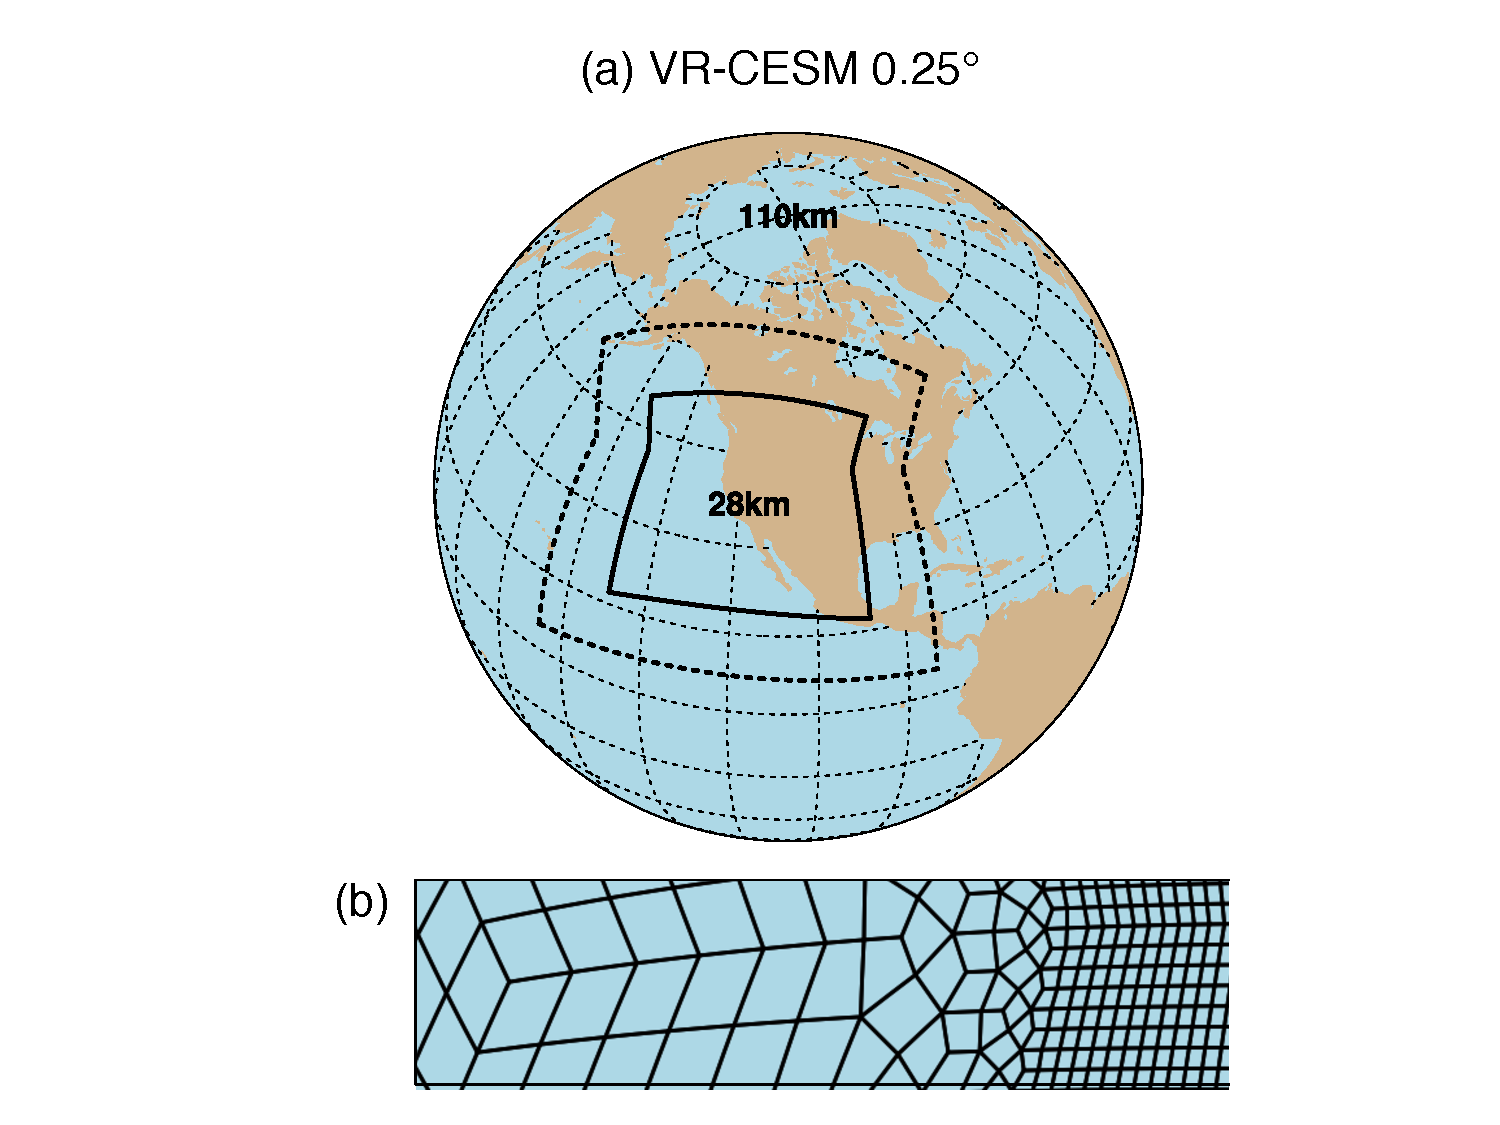
\includegraphics[width=6in]{gridmesh.pdf}
\caption{(a) The approximate grid spacing used for the VR-CESM 0.25$^\circ$ mesh. (b) A depiction of the transition from the global $1^\circ$ resolution mesh through two layers of refinement to $0.25^\circ$.}
\label{fig:Figure 1}
\end{center}
\end{figure}

\begin{figure}
\begin{center}
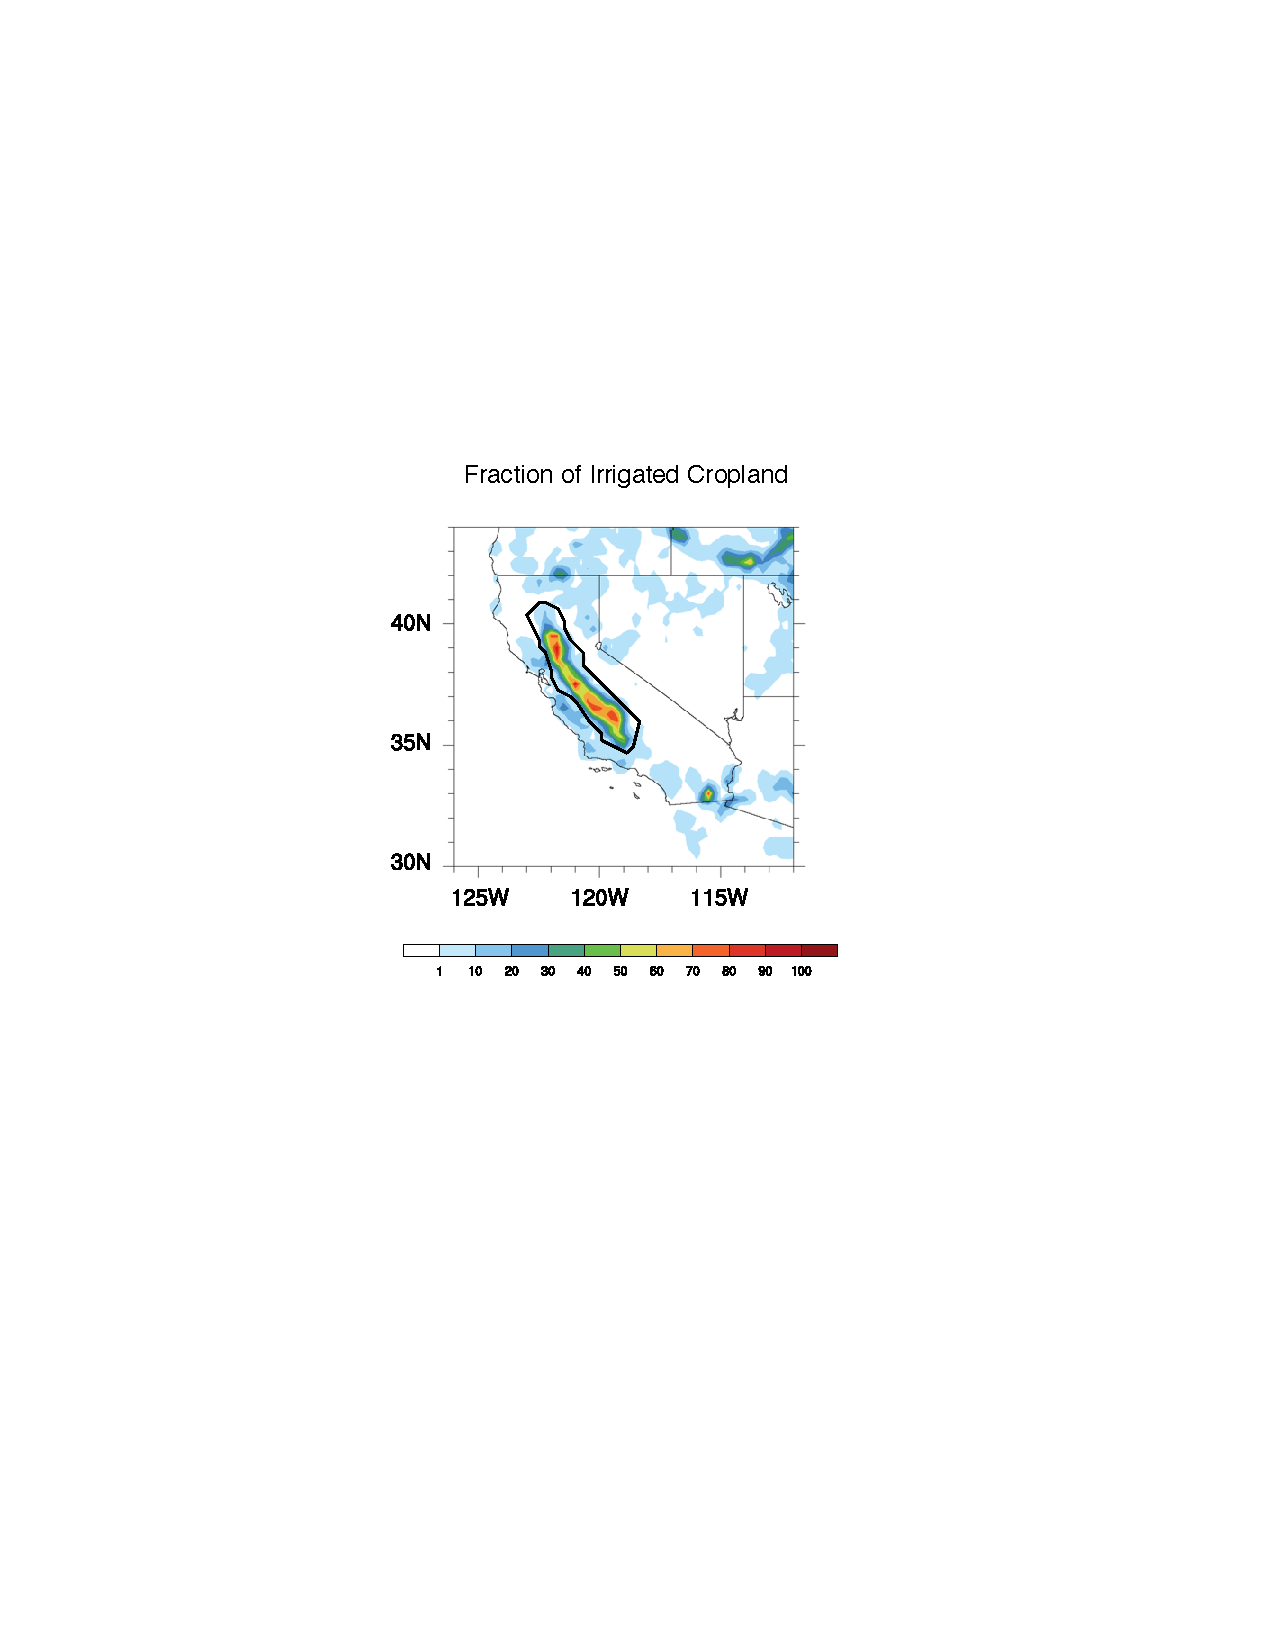
\includegraphics[width=6in]{irrigatedArea.pdf}
\caption{The percent of irrigated cropland at each grid cell.  The black line delineates the boundary of the CV region.}
\label{fig:Figure 2}
\end{center}
\end{figure}

\begin{figure}
\begin{center}
\includegraphics[width=6in]{irrig_2dplot.pdf}
\caption{Average JJA Tmax, Tmin and Tavg over year 1980-2005 for models and observations ($^\circ$C). Hatching denotes statistically significant differences between NRG and IRG.}
\label{fig:Figure 3}
\end{center}
\end{figure}

\begin{figure}
\begin{center}
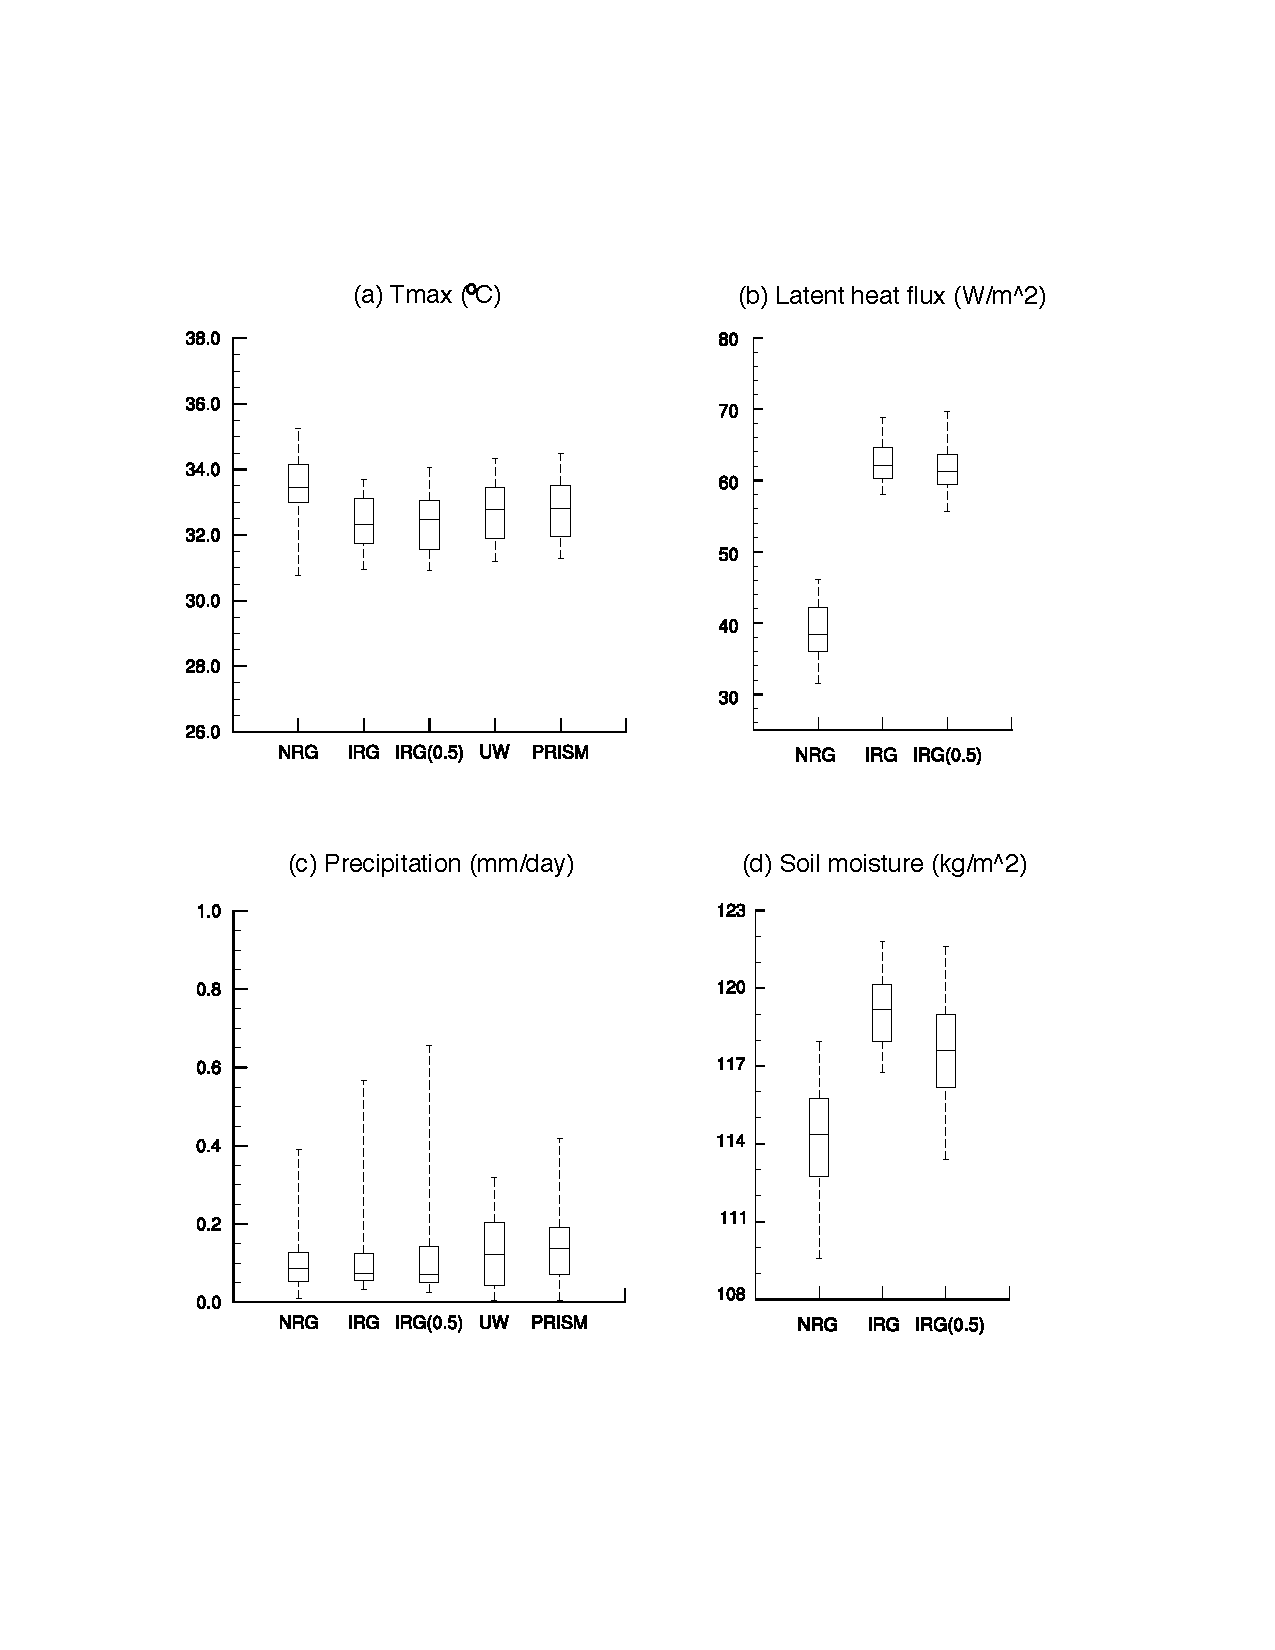
\includegraphics[width=6in]{irrig_boxplot.pdf}
\caption{Box plots for JJA averaged  (a) Tmax, (b) Latent heat flux, (c) Precipitation, and (d) Soil moisture.  From top to bottom, horizontal lines represent maximum value, third quartile, median, first quartile and minimum value, respectively.} 
\label{fig:Figure 4}
\end{center}
\end{figure}


\begin{figure}
\begin{center}
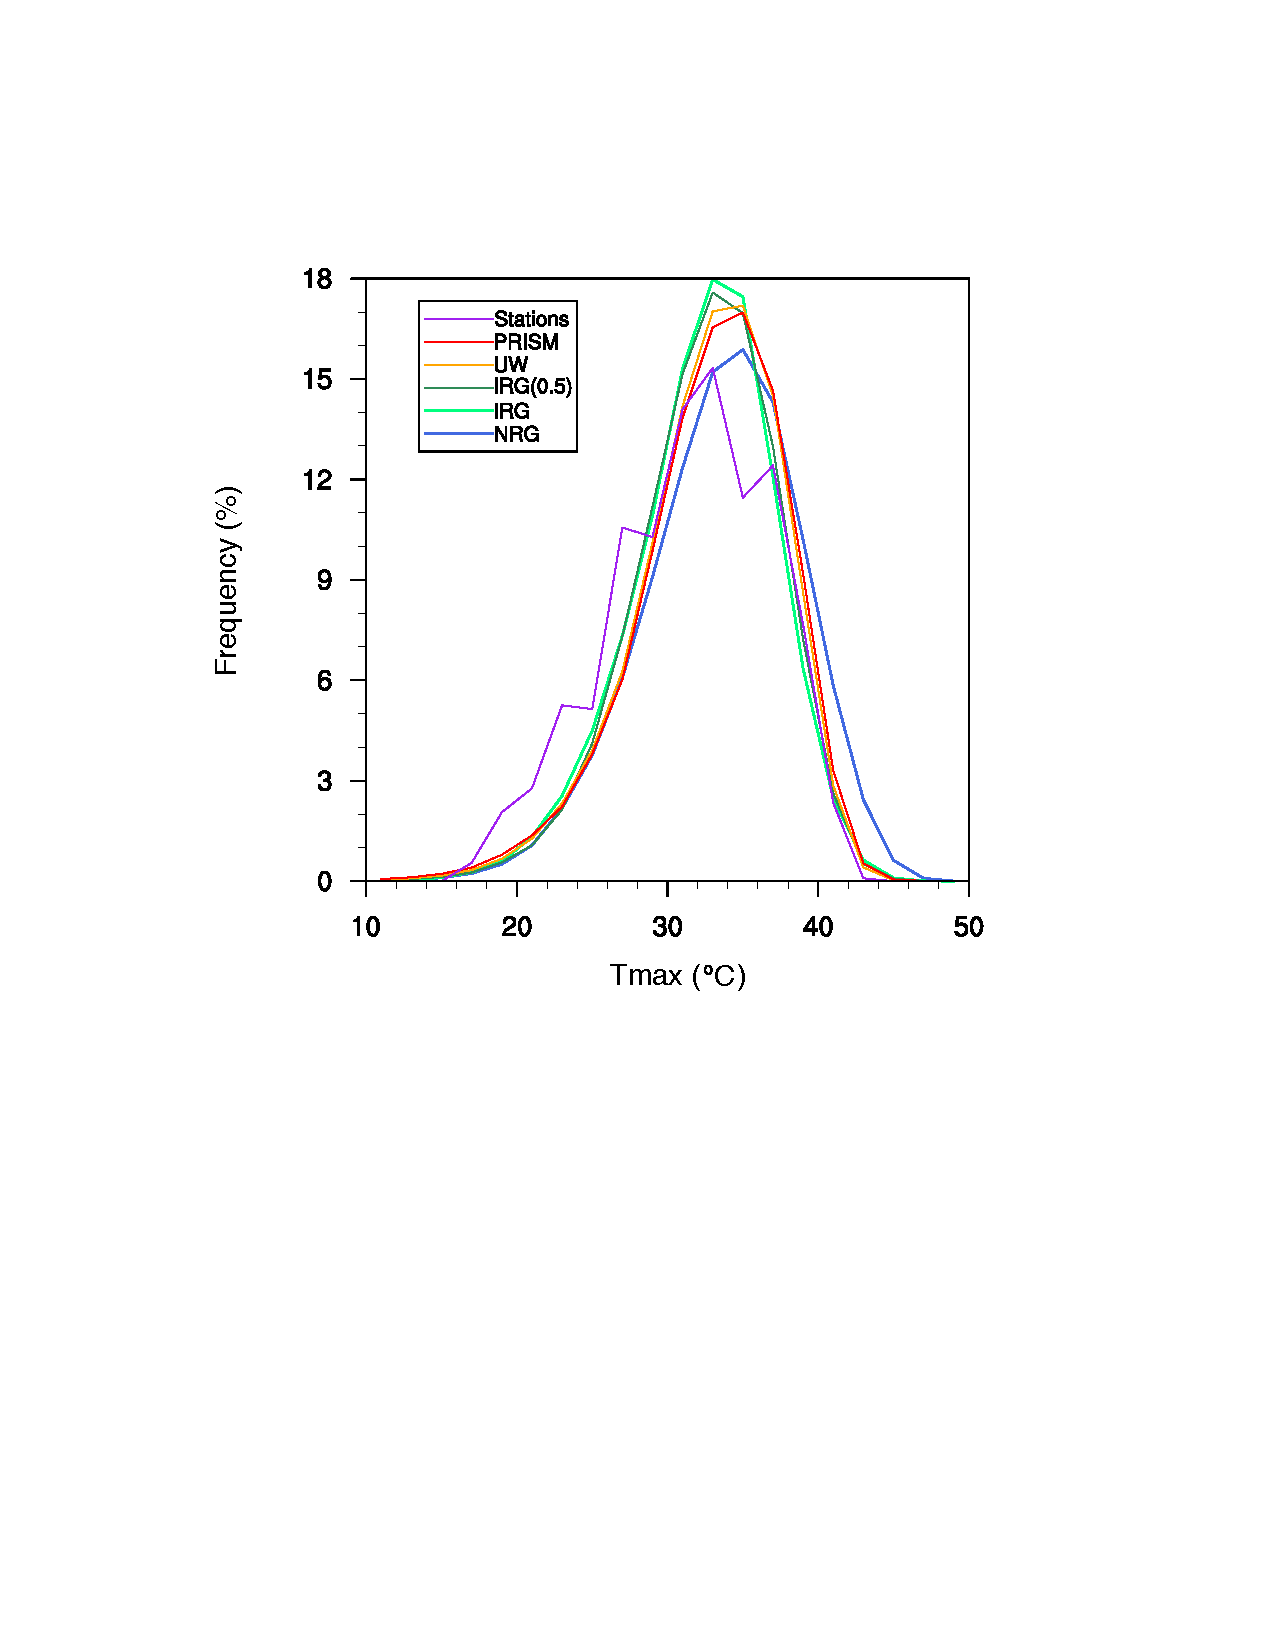
\includegraphics[width=6in]{irrig_pdf.pdf}
\caption{Frequency distribution of JJA daily Tmax over the period 1981-2005 from simulations and reference datasets.}
\label{fig:Figure 5}
\end{center}
\end{figure}

\begin{figure}
\begin{center}
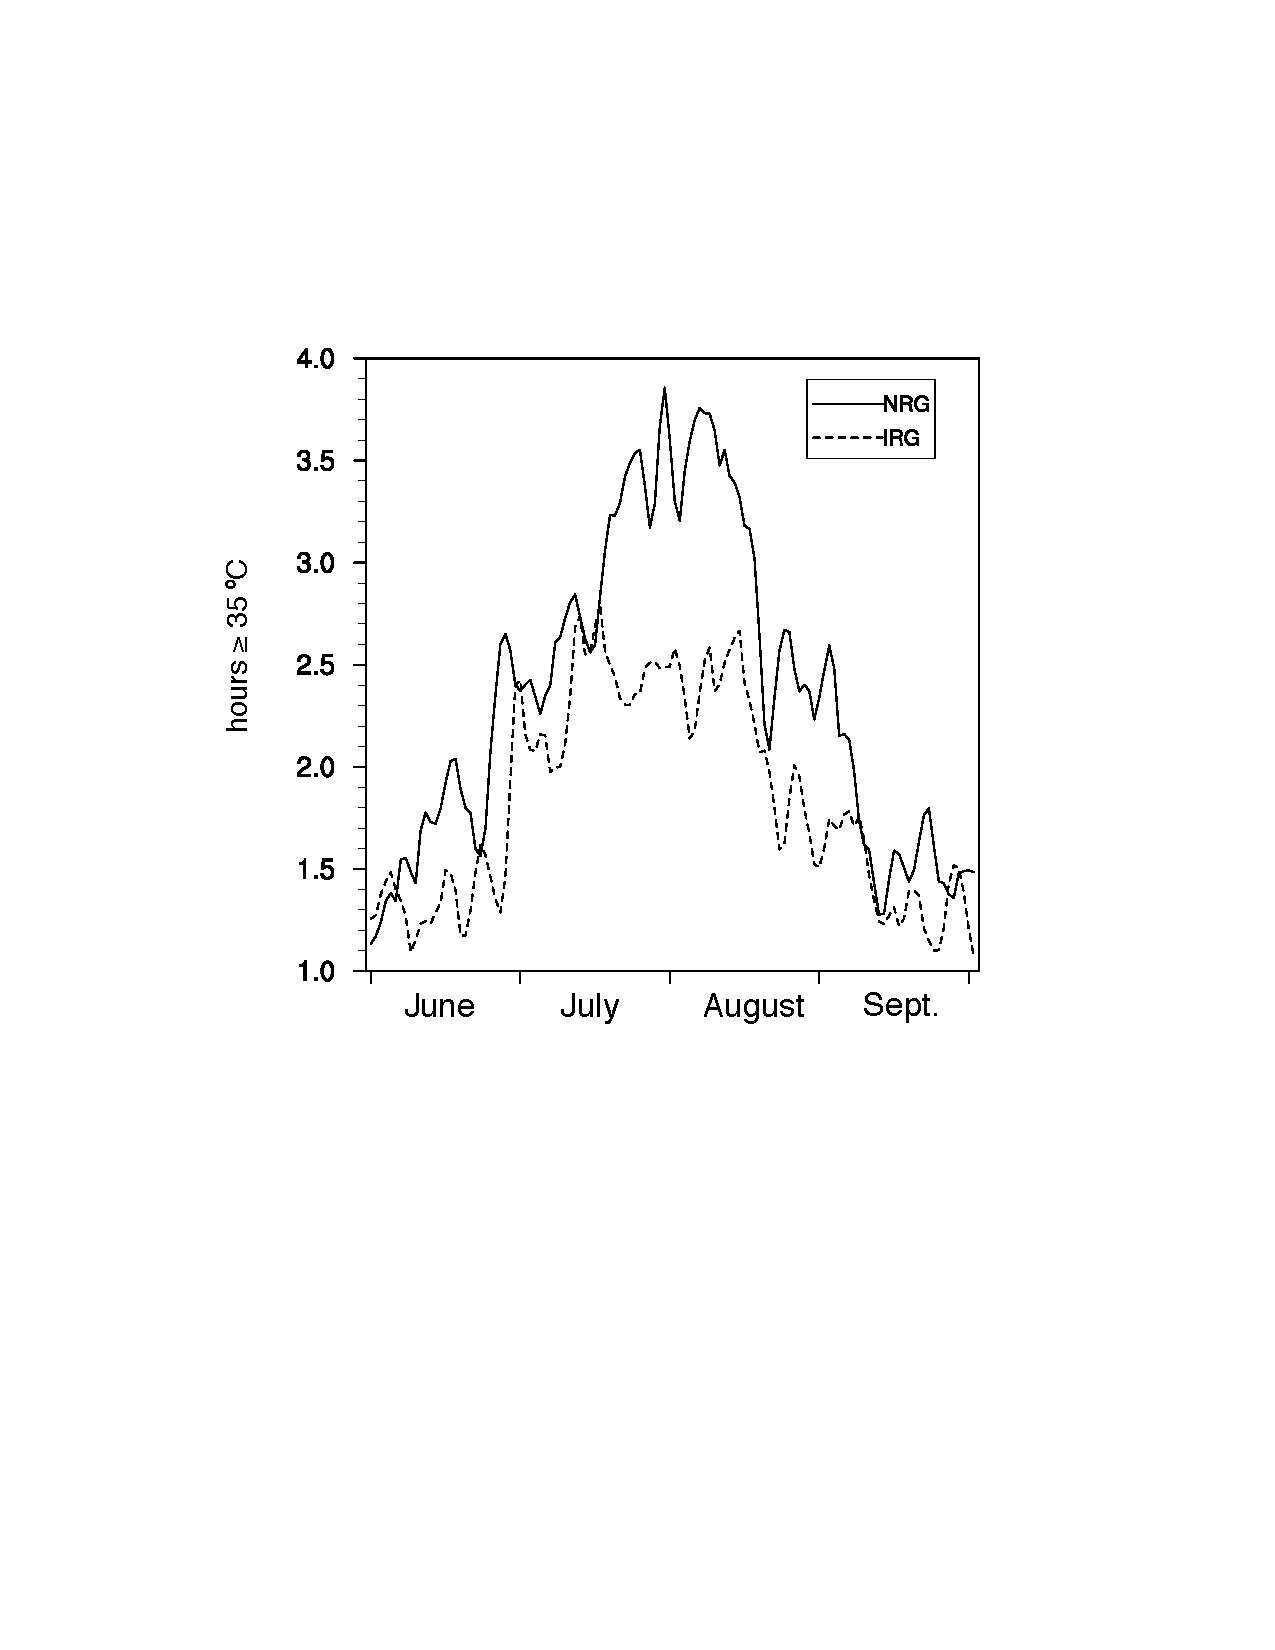
\includegraphics[width=6in]{irrig_hours_T2>=35.pdf}
\caption{The number of hours larger than or equal to 35$^\circ$C per day from June 1st to September 30th averaged over 1980-2005, for NRG and IRG runs.}
\label{fig:Figure 6}
\end{center}
\end{figure}

\end{document}